\documentclass[../../main.tex]{subfiles}

\begin{document}
\problem{17: To setup the connection, how many UDP datagrams are exchanged between your computer and the server? Explain your answer.}
\begin{wts}
To setup the connection, how many UDP datagrams are exchanged between your computer and the server? Explain your answer.
\end{wts}
\begin{proof}
\subfile{./Folland/Theorem4_2}
\newcommand{\pxf}{P_{\mathbf{X}}(f)}
\newcommand{\pyf}{P_{\mathbf{y}}(f)}
\newcommand{\hf}{\mathbf{H}(f)}
\newcommand{\xf}{\mathbf{X}(f)}
\newcommand{\yf}{\mathbf{Y}(f)}
\subsection*{B1 Signal Sizes}
We begin with mathematical definitions.
\begin{definition}
    Energy of a signal $x(t)\iff \bf{X}(f)$ is a non-negative quantity,
    \begin{align*}
        E_x&=\int |x|^2dt = \norm{x}_2^2\\
        E_x&= \int |\bf{X}|^2df = \norm{\bf{X}}_2^2
    \end{align*}
    It has units of J.
\end{definition}
\begin{definition}
    Power Spectral Density of a signal $x(t)\iff \bf{X}(f)$ is a function,
    \[
    P_{\mathbf{X}}:\Omega\to\mathbb{R},\quad P_{\mathbf{X}} (f) = \lim_{d\to\infty} \dfrac{|\mathbf{X}_d (f)|^2}{d}
    \]
    where $\mathbf{X}_d (f) = \cal{F}\biggl\{x(t)\chi_{\left[-\frac{d}{2},+\frac{d}{2}\right]}\biggr\}$. $P_{\mathbf{X}}$ has units W/Hz. Other names are:
    \begin{itemize}
        \item Power Spectrum, and
        \item Signal Power distribution in the frequency domain.
    \end{itemize}
\end{definition}
\begin{definition}
    Energy Spectral Density of a signal $x(t)\iff \mathbf{X}(f)$ is a function,
    \[
    |\mathbf{X}(f)|^2: \Omega\to\mathbb{R},
    \]
    It has units J/Hz. Other names are:
    \begin{itemize}
        \item Energy Spectrum, and
        \item Signal energy distribution in the frequency domain.
    \end{itemize}
\end{definition}
\begin{definition}
    Power of a signal $x(t)\iff \bf{X}(f)$ is a quantity
    \begin{align*}
    P_x &= \lim_{d\to\infty}d^{-1}\int|x(t)|^2\chi_{\left[-\frac{d}{2},+\frac{d}{2}\right]}dt\\[2ex]
    P_x &= \int P_{\mathbf{X}}df = \int \lim_{d\to\infty}\dfrac{|\mathbf{X}_d(f)|^2}{d}df
    \end{align*}
    For a sinusoid in $x(t)=A\cos(2\pi f_c t+\theta)$, $P_x=A/2$. It has units of W.
\end{definition}
\begin{remark}
    One should not conflate Power with Power Spectral Density, one is a quantity and the other is a function.
\end{remark}
An alternate characterisation of the Power of a signal would be to use the average function for some $|x(t)|^2\in L^1_{loc}$
\[
P_x=\lim_{r\to\infty}A_r(x(0))=\dfrac{1}{m(B(r,0))}\int_{B(r,0)}|x(t)|^2dt
\]
\begin{definition}
    The absolute bandwidth $B$ of a signal is 
    \[
    \mu(\supp{S(f)}\cap\mathbb{R}^+)=\mu\left(\bigcap\{[a,b],\,0\leq a\leq b,\,\supp{S(f)\subseteq[a,b]}\}\right)
    \]
\end{definition}
\begin{definition}
    If the smallest closed interval that contains $\supp{S(f)}\cap\mathbb{R}^+$ is given by $[f_1,f_2]$, then the center frequency $f_0$ of $s(t)$ is
    \[
    f_0 = (f_2-f_1)/2
    \]
\end{definition}
\begin{definition}
    A bandlimited signal is one with compact support in the frequency domain. In symbols, $\xf\in C_c(\Omega)$.
\end{definition}
\begin{definition}
    A strictly bandlimited, real-valued signal is called a baseband signal if and only if $f_0=0$.
\end{definition}
\begin{wtr}

\end{wtr}
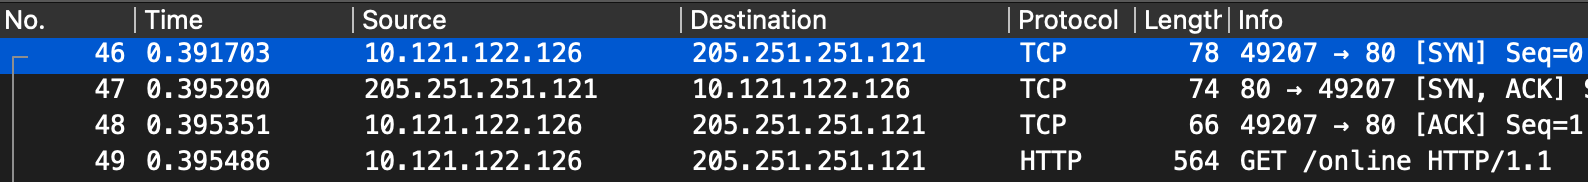
\includegraphics[width=\textwidth]{subfiles/images/ECSE_308_Lab_5_1_SUPA_PAGE1_0_Image27.png}
\end{proof}

\end{document}